\chapter{Como os animais respiram}\label{ch:g7:how-animals-breathe}

A truta debaixo da ponte, a minhoca debaixo do gramado, a libélula
acima dele e você em cima dele estão todos fazendo a mesma coisa neste
minuto: retirando \omterm{def:g7:what-is-respiration:respiration}{oxigênio} do que está em volta
(\cref{def:g7:what-is-respiration:respiration}). Mas o que está em
volta de cada um é diferente --- ar, \omterm{def:g6:decomposers-and-soil:soil}{solo}, água --- e o equipamento
também. Este capítulo é uma visita às máquinas respiratórias do reino
\omterm{def:g1:animals-around-us:animal}{animal}.

\section{Um problema, quatro máquinas}

\begin{proposition}[A especificação comum]\label{prop:g7:how-animals-breathe:spec}
Todo órgão respiratório, seja de quem for, é construído segundo uma
única especificação, já encontrada na
\cref{rem:g4:breathing:sponge}: uma superfície \emph{grande},
\emph{fina} e \emph{úmida} onde o \omterm{prop:g4:journey-of-food:absorb}{sangue} do \omterm{def:g1:animals-around-us:animal}{animal} (ou o líquido do
corpo dele) chega perto o bastante do que está em volta para o
\omterm{def:g7:what-is-respiration:respiration}{oxigênio} atravessar para dentro e o \omterm{def:g7:what-is-respiration:respiration}{gás carbônico} para fora. Grande
para haver travessia suficiente; fina para a travessia ser fácil;
úmida porque os gases atravessam dissolvidos. As máquinas diferem no
jeito de manter essa superfície voltada para o meio.
\end{proposition}
\admitted

\begin{definition}[As quatro máquinas]\label{def:g7:how-animals-breathe:four}
Os \omterm{def:g1:animals-around-us:animal}{animais} mantêm as superfícies de troca deles de quatro jeitos
principais:
\begin{enumerate}
  \item \emph{pulmões}\index{pulmão}: bolsas cheias de ar dobradas
        \emph{dentro} do corpo, ventiladas por movimentos
        respiratórios --- \omterm{prop:g3:sorting-living-things:groups}{mamíferos}, \omterm{prop:g3:sorting-living-things:groups}{aves}, \omterm{prop:g4:classifying-animals:classes}{répteis}, \omterm{prop:g3:sorting-living-things:groups}{anfíbios} adultos;
  \item \emph{brânquias}\index{brânquia}: superfícies emplumadas
        mantidas \emph{fora do corpo ou na borda dele}, lavadas por
        uma corrente de água --- \omterm{prop:g3:sorting-living-things:groups}{peixes}
        (\cref{exo:g4:breathing:11}), \omterm{ex:g2:animals-grow-up:frog}{girinos}, muitas larvas
        aquáticas, mexilhões;
  \item \emph{traqueias}\index{traqueia (inseto)}: uma rede de tubos
        finos de ar canalizados de aberturas ao longo do corpo direto
        para cada órgão --- os \omterm{prop:g3:sorting-living-things:groups}{insetos}; o ar é entregue de porta em
        porta, quase sem a ajuda do \omterm{prop:g4:journey-of-food:absorb}{sangue};
  \item \emph{respiração pela pele}\index{respiração pela pele}: a
        \omterm{def:g1:the-five-senses:sense}{pele} úmida inteira como superfície de troca --- a minhoca
        inteiramente; os \omterm{prop:g3:sorting-living-things:groups}{anfíbios} como um grande complemento aos
        pulmões simples deles.
\end{enumerate}
\end{definition}

\begin{example}[Observando as máquinas em funcionamento]\label{ex:g7:how-animals-breathe:watch}
Cada máquina mostra o ritmo dela. A boca e os opérculos da truta
bombeiam numa alternância constante --- água entrando pela boca,
passando pelas \omterm{def:g7:how-animals-breathe:four}{brânquias}, saindo por baixo dos opérculos. O abdome do
gafanhoto em repouso pulsa --- bombeando os tubos de ar dele. A
garganta do sapo palpita --- empurrando ar para os \omterm{def:g7:how-animals-breathe:four}{pulmões} dele (sem
caixa torácica para fazer isso). Só a minhoca não mostra nada: a
\omterm{def:g7:how-animals-breathe:four}{respiração pela pele} não tem movimento nenhum, e é justamente por isso
que a \cref{def:g7:what-is-respiration:respiration} distinguiu a troca
do bombeamento.
\end{example}

\begin{omfigure}
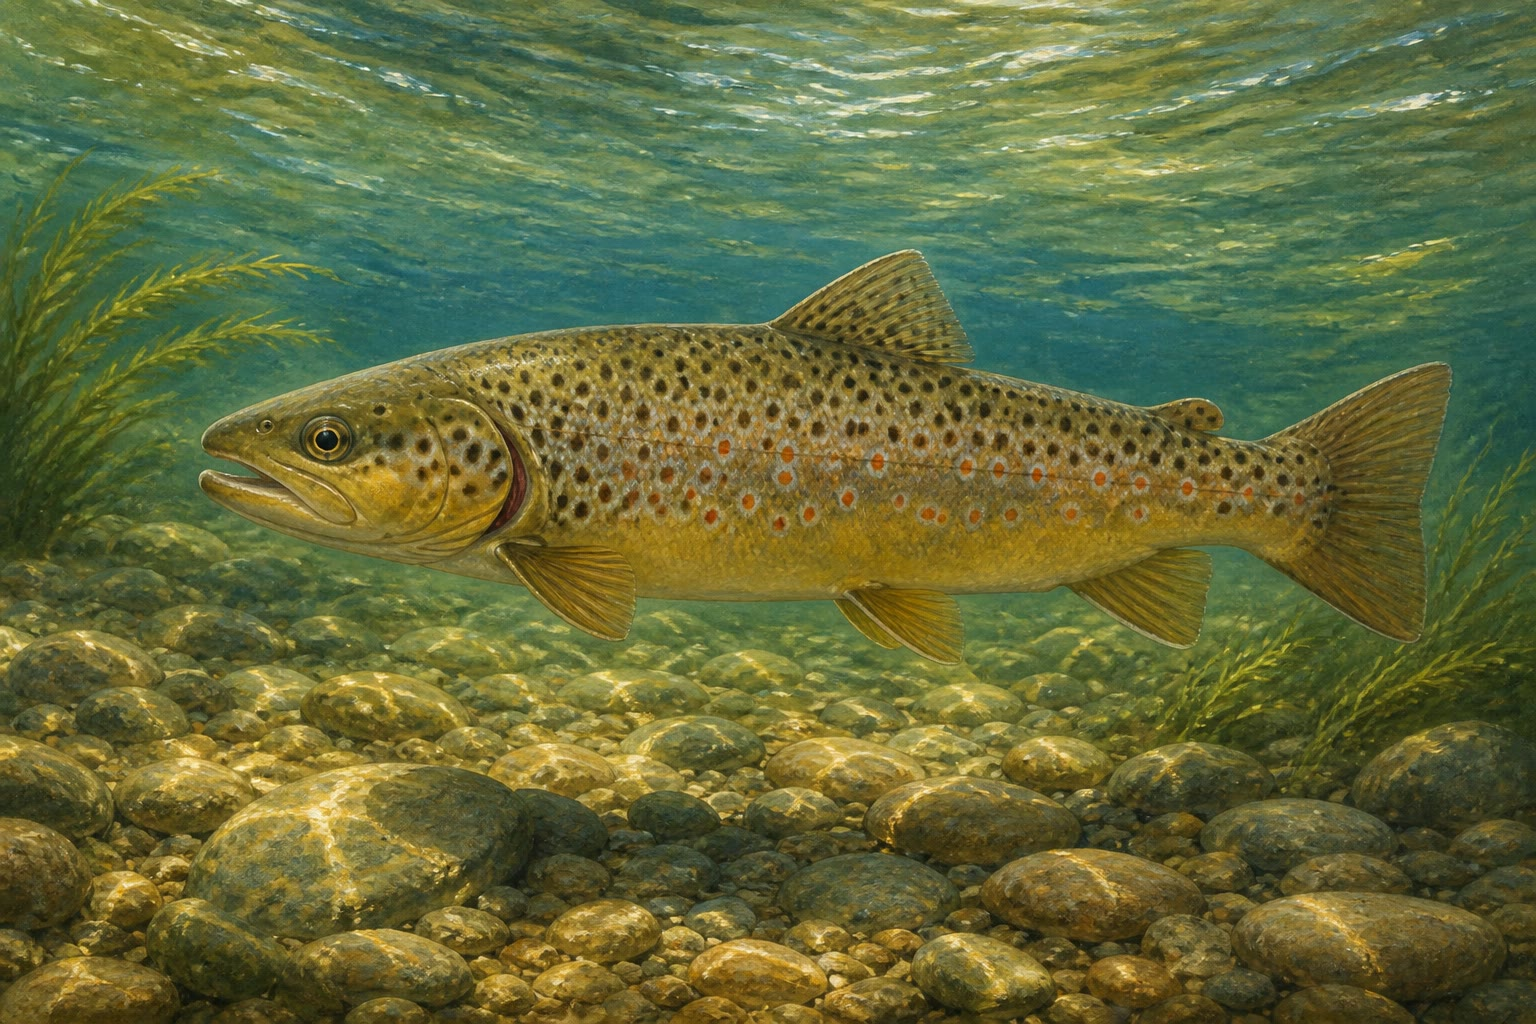
\includegraphics[width=0.6\linewidth]{images/book1/ai/g7-breathe-trout.jpg}

{\small O dono da máquina de \omterm{def:g7:how-animals-breathe:four}{brânquias} em posto: a boca e os
opérculos bombeando a corrente de mão única que lava as superfícies de
troca emplumadas dele.}
\end{omfigure}

\begin{omfigure}
\begin{tikzpicture}
  \node[anchor=south west, inner sep=0] (img) at (0,0)
    {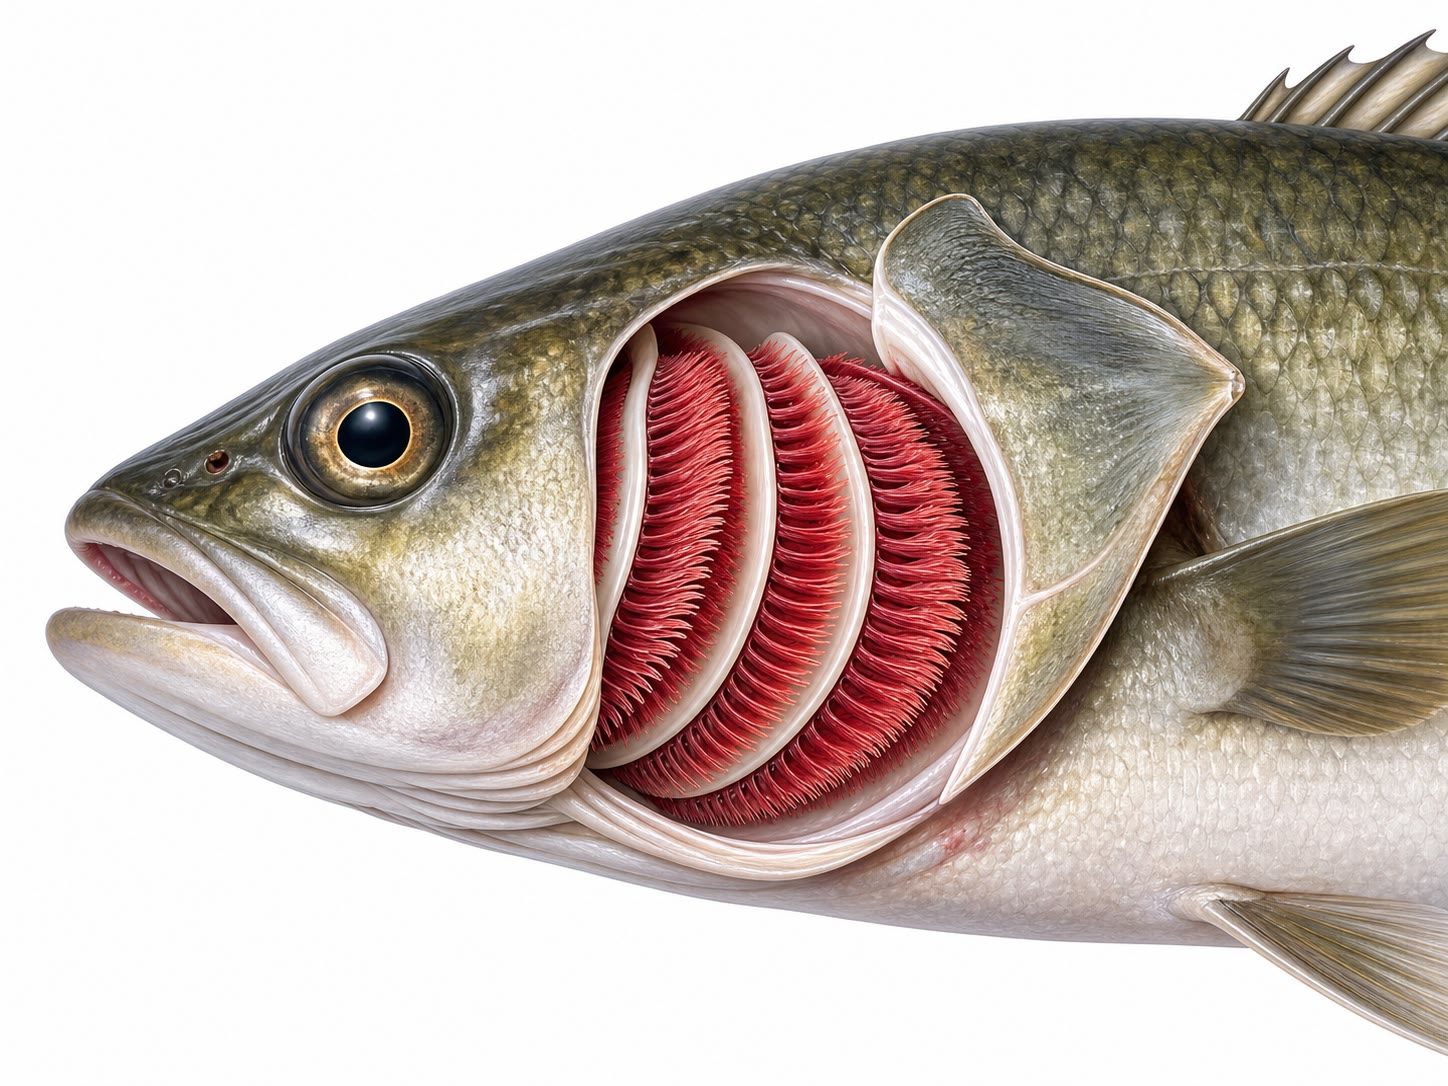
\includegraphics[width=0.56\linewidth]{images/book1/ai/fig-fish-gills.jpg}};
  \begin{scope}[x={(img.south east)}, y={(img.north west)},
      every node/.style={font=\small}]
    \draw[omDef, thick] (0.55,0.64) -- (0.32,0.92)
      node[above, align=center] {as brânquias emplumadas,\\ lavadas pela corrente};
    \draw[->, very thick, omDef] (-0.17,0.40) -- (0.02,0.40);
    \node[left, omDef] at (-0.18,0.40) {entra água};
    \draw[->, very thick, omDef] (0.62,0.26) to[bend left=10] (0.70,-0.04);
    \node[below, omDef, align=center] at (0.70,-0.05)
      {sai água, por baixo\\ do opérculo levantado};
  \end{scope}
\end{tikzpicture}

{\small A máquina de \omterm{def:g7:how-animals-breathe:four}{brânquias}, destampada: uma corrente de mão única
entra pela boca, lava os arcos branquiais vermelhos e emplumados e sai
por baixo do opérculo.}
\end{omfigure}

\section{A máquina combina com o meio --- e com a vida}

\begin{proposition}[Por que cada máquina em cada lugar]\label{prop:g7:how-animals-breathe:fits}
As máquinas se encaixam nos meios e nas vidas
(\cref{def:g4:adapted-to-their-world:adaptation} em ação sobre a
\omterm{def:g7:what-is-respiration:respiration}{respiração}):
\begin{itemize}
  \item as \omterm{def:g7:how-animals-breathe:four}{brânquias} servem à água: as superfícies emplumadas delas
        se abrem flutuando nela, lavadas o tempo todo --- e desabam
        inúteis no ar (a truta sufocando do
        \cref{exo:g4:breathing:11});
  \item os \omterm{def:g7:how-animals-breathe:four}{pulmões} servem ao ar: dobrados por dentro, eles continuam
        úmidos onde a água aberta se perderia --- mas não conseguem
        colher o \omterm{def:g7:what-is-respiration:respiration}{oxigênio} dissolvido e escasso da água;
  \item as \omterm{def:g7:how-animals-breathe:four}{traqueias} servem a corpos pequenos: excelentes em
        distâncias de milímetros, elas entregam devagar demais em
        distâncias longas --- um dos motivos de os \omterm{prop:g3:sorting-living-things:groups}{insetos} continuarem
        pequenos;
  \item a \omterm{def:g7:how-animals-breathe:four}{respiração pela pele} serve a vidas pequenas e de \omterm{def:g1:the-five-senses:sense}{pele} úmida
        em lugares úmidos: a superfície inteira da minhoca mal atende
        o corpo fino dela, e o ar seco a mata --- lembre das minhocas
        encalhadas depois da chuva.
\end{itemize}
\end{proposition}
\admitted

\begin{example}[Duas vidas, duas máquinas num animal só]\label{ex:g7:how-animals-breathe:frog}
O sapo percorre o capítulo inteiro numa vida só: \omterm{def:g7:how-animals-breathe:four}{brânquias} enquanto
girino (a máquina de quem mora na água,
\cref{ex:g2:animals-grow-up:frog}), \omterm{def:g7:how-animals-breathe:four}{pulmões} mais \omterm{def:g1:the-five-senses:sense}{pele} úmida quando
adulto --- com os \omterm{def:g7:how-animals-breathe:four}{pulmões} simples e a \omterm{def:g1:the-five-senses:sense}{pele} fazendo boa parte do
trabalho, principalmente no inverno frio no fundo da lagoa (o
\cref{exo:g6:life-through-seasons:11}: aquele sapo dormente respira só
pela \omterm{def:g1:the-five-senses:sense}{pele}). A \omterm{def:g2:animals-grow-up:metamorphosis}{metamorfose} reconstrói até a maquinaria respiratória.
\end{example}

\begin{example}[Respirar ar vivendo na água]\label{ex:g7:how-animals-breathe:airinwater}
Quem mora na água e tem \omterm{def:g7:how-animals-breathe:four}{pulmões} precisa fazer o trajeto de ida e
volta. O golfinho e a baleia sobem para soprar e inspirar
(\cref{ex:g6:classification-kinship:whale}: \omterm{def:g7:how-animals-breathe:four}{pulmões} de mamífero,
herdados de ancestrais terrestres); o caramujo de lagoa sobe até a
superfície para reabastecer; o besouro mergulhador carrega uma bolha
prateada de ar debaixo das asas duras --- um cilindro de mergulho,
renovado na superfície. O \omterm{def:g2:where-animals-live:habitat}{hábitat} é negociável; o meio da máquina não é.
\end{example}

\begin{method}[Ler a respiração de um animal]\label{met:g7:how-animals-breathe:read}
Diante de um \omterm{def:g1:animals-around-us:animal}{animal} desconhecido:
\begin{enumerate}
  \item onde ele vive --- e ele pode sair de lá? (água, ar, \omterm{def:g6:decomposers-and-soil:soil}{solo};
        morador ou visitante que faz o trajeto);
  \item procure os sinais da máquina: opérculos ou tufos emplumados;
        narinas e um peito que se mexe; fileiras de aberturas
        minúsculas ao longo do corpo de um inseto; ou nada visível,
        além de uma \omterm{def:g1:the-five-senses:sense}{pele} úmida;
  \item observe o ritmo: opérculos bombeando, abdome pulsando, peito
        subindo, visitas à superfície;
  \item diga o nome da máquina --- e confira essa máquina com o meio,
        usando a \cref{prop:g7:how-animals-breathe:fits}.
\end{enumerate}
\end{method}

\begin{remark}[A especificação nunca muda]\label{rem:g7:how-animals-breathe:same}
Por baixo da variedade, examine de perto qualquer uma das quatro
máquinas e a \cref{prop:g7:how-animals-breathe:spec} reaparece: as
plumas da \omterm{def:g7:how-animals-breathe:four}{brânquia}, as bolsas do \omterm{def:g7:how-animals-breathe:four}{pulmão}, as pontas mais finas das
\omterm{def:g7:how-animals-breathe:four}{traqueias} e a \omterm{def:g1:the-five-senses:sense}{pele} da minhoca são todas pontos de encontro grandes,
finos e úmidos entre o meio e o corpo. Quatro máquinas, uma
especificação --- a \omterm{prop:g5:first-look-at-cells:principle}{unidade da vida}
(\cref{prop:g5:first-look-at-cells:principle}), escrita em equipamento
respiratório.
\end{remark}

\section{Exercícios}

\begin{exercise}[$\star$]\label{exo:g7:how-animals-breathe:1}
Enuncie a especificação comum que todo órgão respiratório cumpre e por
que cada uma das três propriedades dela importa.
\end{exercise}

\begin{exercise}[$\star$]\label{exo:g7:how-animals-breathe:2}
Diga as quatro máquinas, cada uma com dois donos.
\end{exercise}

\begin{exercise}[$\star$]\label{exo:g7:how-animals-breathe:3}
Descreva o bombeamento da truta: o caminho da água ao entrar, ao
atravessar e ao sair.
\end{exercise}

\begin{exercise}[$\star$]\label{exo:g7:how-animals-breathe:4}
Como os \omterm{prop:g3:sorting-living-things:groups}{insetos} entregam \omterm{def:g7:what-is-respiration:respiration}{oxigênio} sem \omterm{def:g7:how-animals-breathe:four}{pulmões} --- e quase sem a ajuda
do \omterm{prop:g4:journey-of-food:absorb}{sangue}?
\end{exercise}

\begin{exercise}[$\star$]\label{exo:g7:how-animals-breathe:5}
Por que uma truta encalhada sufoca num ar rico em \omterm{def:g7:what-is-respiration:respiration}{oxigênio}?
\end{exercise}

\begin{exercise}[$\star$]\label{exo:g7:how-animals-breathe:6}
Por que o sol seco mata uma minhoca na calçada? Que máquina falha, e
como?
\end{exercise}

\begin{exercise}[$\star\star$]\label{exo:g7:how-animals-breathe:7}
Liste as máquinas respiratórias do sapo ao longo da vida dele, cada
uma com a estação ou a etapa correspondente.
\end{exercise}

\begin{exercise}[$\star\star$]\label{exo:g7:how-animals-breathe:8}
O golfinho vive como um peixe, mas se afoga como um homem. Explique
com a máquina e com a ancestralidade
(\cref{ex:g6:classification-kinship:whale}).
\end{exercise}

\begin{exercise}[$\star\star$]\label{exo:g7:how-animals-breathe:9}
O que é a bolha prateada do besouro mergulhador, e o que o besouro
precisa fazer com ela regularmente?
\end{exercise}

\begin{exercise}[$\star\star$]\label{exo:g7:how-animals-breathe:10}
Rode o \cref{met:g7:how-animals-breathe:read} em: (a) um mexilhão;
(b) um gafanhoto; (c) uma cobra-d'água atravessando a lagoa a nado.
\end{exercise}

\begin{exercise}[$\star\star$]\label{exo:g7:how-animals-breathe:11}
Por que não existem \omterm{prop:g3:sorting-living-things:groups}{insetos} do tamanho de uma baleia? Responda com o
limite das \omterm{def:g7:how-animals-breathe:four}{traqueias}.
\end{exercise}

\begin{exercise}[$\star\star\star$]\label{exo:g7:how-animals-breathe:12}
``Quatro máquinas, uma especificação.'' Defenda a frase: diga a
especificação compartilhada e mostre como a \omterm{def:g7:how-animals-breathe:four}{brânquia}, o \omterm{def:g7:how-animals-breathe:four}{pulmão}, as
\omterm{def:g7:how-animals-breathe:four}{traqueias} e a \omterm{def:g1:the-five-senses:sense}{pele} atendem cada uma às três exigências dela.
\end{exercise}

\section{Problema: O censo dos respiradores da lagoa}

\begin{problem}[{Problema de fim de semana --- uma lagoa, todas as
máquinas em ação}]\label{pb:g7:how-animals-breathe:1}
Uma tarde na lagoa com rede, caixa de observação e caderno. O censo:
alevinos de truta e peixinhos-espinho; \omterm{ex:g2:animals-grow-up:frog}{girinos} (alguns com as \omterm{def:g1:my-body:parts}{pernas}
de trás); sapos adultos; caramujos de lagoa passeando pela película da
superfície; um besouro mergulhador lampejando prateado; larvas de
efêmera com tufos emplumados debaixo das pedras; e, no gramado úmido
do barranco, minhocas.

\medskip\noindent\textbf{Parte I --- Dando nome às máquinas.}
\begin{enumerate}
  \item Atribua a cada \omterm{def:g1:my-body:parts}{membro} do censo a máquina respiratória dele.
  \item Os tufos emplumados da larva de efêmera se agitam sem parar,
        mesmo em água parada. O que são esses tufos, e para que serve
        a agitação?
  \item Que \omterm{def:g1:my-body:parts}{membros} do censo precisam visitar a superfície, e por que
        exatamente esses?
  \item Os \omterm{ex:g2:animals-grow-up:frog}{girinos} sem \omterm{def:g1:my-body:parts}{pernas} e os com \omterm{def:g1:my-body:parts}{pernas} podem diferir por
        dentro tanto quanto por fora. Que reconstrução está em
        andamento, segundo o \cref{ex:g7:how-animals-breathe:frog}?
\end{enumerate}

\medskip\noindent\textbf{Parte II --- As máquinas sob
tensão.}
\begin{enumerate}[resume]
  \item Uma semana quente e sem vento baixa o \omterm{def:g7:what-is-respiration:respiration}{oxigênio} dissolvido da
        lagoa (o \cref{ch:g7:oxygen-in-the-water} vai explicar por
        quê). Ponha o censo em ordem: quem sofre primeiro --- quem usa
        \omterm{def:g7:how-animals-breathe:four}{brânquias} ou quem faz o trajeto até a superfície? Por quê?
  \item Naquela semana, os peixinhos-espinho ficam logo abaixo da
        superfície, com a boca trabalhando na película. Interprete o
        comportamento com a especificação: o que o milímetro de cima
        da água tem de especial?
  \item Alguém entra na água sem cuidado e levanta nuvens de lama
        fina. Que máquina entope, e o que você esperaria que os
        \omterm{def:g1:animals-around-us:animal}{animais} afetados fizessem?
  \item Depois de uma noite de chuva, as minhocas do gramado ficam
        deitadas no caminho. Explique essa cena clássica: que máquina
        e que condição as empurraram para cima?
\end{enumerate}

\medskip\noindent\textbf{Parte III --- O mapa maior.}
\begin{enumerate}[resume]
  \item Monte o censo como uma tabela: \omterm{def:g1:animals-around-us:animal}{animal}, máquina, meio, morador
        ou visitante que faz o trajeto. Que especificação única
        encabeça toda \omterm{def:g3:bones-and-muscles:skeleton}{coluna} de máquina, segundo a
        \cref{rem:g7:how-animals-breathe:same}?
  \item A lagoa congela na superfície em janeiro, lacrando a
        superfície. Preveja os destinos de inverno: os sapos
        (\cref{exo:g6:life-through-seasons:11}), os caramujos, o
        besouro, os \omterm{prop:g3:sorting-living-things:groups}{peixes} --- quem fica em apuros e quem está
        garantido?
  \item Chega um recém-chegado: uma aranha-d'água que tece um sino de
        seda e o abastece com ar da superfície. Ponha o truque dela ao
        lado do truque do besouro e diga a máquina que ela continua
        servindo.
  \item Conclua: por que uma lagoa pequena precisa de quatro máquinas
        respiratórias diferentes para ser habitada por inteiro? Uma
        frase, usando \emph{meio} e \emph{\omterm{def:g7:what-is-respiration:respiration}{oxigênio}}.
\end{enumerate}
\end{problem}
